\documentclass{deliverablereport}

\usepackage{pdfpages}
\usepackage{multirow}
\usepackage{doi}
\usepackage{hyperref}
\hypersetup{
  colorlinks=true,
  urlcolor=cyan,
  linkcolor=blue,
  citecolor=blue,
}

\usepackage{natbib}

\deliverable{hpc}{LinBox-algo}
\deliverydate{31/08/2018}
\duedate{31/08/2018 (M36)}
\author{Cl\'ement Pernet and Jean-Guillaume Dumas}

\begin{document}
\maketitle
% This will be the abstract, fetched from the github description
\githubissuedescription

% write the report here
%%%%%%%%%%%%%%%%%%%%%%%%%%%%%%%%%ù
\section{Algorithmic innovations}

\subsection{Dense Gaussian elimination}

Gaussian elimination is among the most commonly used computing kernel in both
numerical and exact linear algebra, as it is used for solving linear systems,
and more specifically in exact linear algebra for computing nullspace basis,
rank and rank profiles, determinants, characteristic polynomials, etc.

\paragraph{Rank deficient LU decomposition} Before the start of the project, we had a series of contributions in the
development of fast Gaussian elimination algorithms in the context of exact
linear algebra, namely
\begin{enumerate}
\item identifying and connecting all triangular matrix decomposition, revealing
  a crucial invariant, the rank profile, and echelon forms.
\item proposing block recursive (by slab or tile splitting) algorithms computing
  these factorization in the best known time complexities, and without
  additional memory footprint;
\item introducing a new matrix invariant, the rank profile matrix, summarizing
  all information on the row and column rank profiles of the matrix and of all
  of its leading submatrices;
\item a block recursive and a base case iterative algorithm which implementation
  in \texttt{fflas-ffpack} sets the state of the art in terms of computing
  efficiency in sequential and parallel multithreaded contexts, and competes
  with the efficiency of the equivalent numerical Gaussian elimination routine;
\item an exhaustive study of the required
conditions on the pivoting strategy for a Gaussian elimination algorithm to
reveal the rank profile matrix invariant.

\end{enumerate}
A first contribution to this deliverable, published in~\cite{DPS17},
improves over the previous results on the rank profile matrix in the following
ways:
\begin{enumerate}
\item a new probabilistic algorithms to compute the rank profile matrix
  invariant in  $O\tilde\ (r^\omega + mn)$ instead of $O(mnr^{\omega-2})$;
\item a generalization of the existing algorithms to produce the full row and
  column echelon form of the matrix
\item an exhaustive study on how does the notion of rank profile matrix
  generalizes over arbitrary rings.
\end{enumerate}


\paragraph{Symmetric triangular factorization}
When the input matrix is symmetric, a variety of symmetric factorizations and
algorithms is known, depending on the ability to extract
square roots (for the Cholesky factorization), the rank structure and the
pivoting strategy to be used.

If the block iterative algorithms with partial or full pivoting are well studied
in numerical linear algebra, the recursive block algorithms were only
approached recently and with strong restrictions on the pivoting
strategy\footnote{See for instance 
\href{http://www.netlib.org/lapack/lawnspdf/lawn294.pdf}{LAPACK
  Working Note 294, Dec. 2017}, and references therein.}.
We proposed in \cite{DuPe18} (see Appendix~\ref{app:papers}) a generalization of the Aasen algorithm in a block
recursive structure, producing a LDLT factorization with partial pivoting. In
particular, this algorithm is able to also compute the rank profile matrix
invariant and enjoy a reduction of its time complexity to that of matrix
multiplication: $O(mnr^{\omega-2})$. Experiments, displayed in
Table~\ref{tab:ldlt}
%
\begin{table}[htb]\centering
  \footnotesize
    \begin{tabular}{rrrrrrrrrrr}
  \toprule
  \multirow{3}{*}{$n$} & 
  \multicolumn{4}{c}{Gen. rank prof.} & \multicolumn{2}{c}{Gen. rank prof.} &
  \multicolumn{2}{c}{Random RPM} & \multicolumn{2}{c}{Random RPM}\\
  &\multicolumn{4}{c}{ $r=n$}&\multicolumn{2}{c}{ $r=n$}&
  \multicolumn{2}{c}{ $r=n$}&\multicolumn{2}{c}{ $r=n/2$}\\
  & \texttt{dgetrf} & \texttt{dsytrf} & \texttt{dsytrf\_rk} & \texttt{dsytrf\_aa} & PLUQ & LDLT & PLUQ& LDLT & PLUQ & LDLT\\
  \midrule
$100$   & 1.17e-04 & 1.31e-04 & 1.37e-04 & 9.21e-05 & 4.64e-04 & 3.23e-04 & 5.59e-04 & 5.22e-04 & 3.20e-04 & 3.80e-04\\
$200$   & 3.73e-04 & 4.39e-04 & 5.51e-04 & 4.48e-04 & 1.87e-03 & 8.80e-04 & 2.58e-03 & 1.59e-03 & 1.58e-03 & 1.33e-03\\
$500$   & 3.31e-03 & 3.78e-03 & 4.88e-03 & 3.87e-03 & 1.73e-02 & 5.21e-03 & 2.83e-02 & 9.85e-03 & 1.88e-02 & 7.92e-03\\
$1000$  & 2.19e-02 & 2.09e-02 & 2.58e-02 & 2.05e-02 & 8.84e-02 & 2.30e-02 & 9.95e-02 & 4.01e-02 & 6.27e-02 & 3.18e-02\\
$2000$  & 0.145 & 0.127 & 0.154 & 0.127 & 0.438 & 0.127 & 0.490 & 0.191 & 0.274 & 0.150\\
$5000$  & 2.005 & 1.604 & 1.871 & 1.598 & 3.904 & 1.591 & 3.849 & 1.744 & 2.431 & 1.294\\
$10000$ & 14.948 & 11.981 & 13.396 & 12.008 & 24.115 & 10.904 & 23.985 & 11.209 & 14.775 & 7.894\\
  \bottomrule 
  \end{tabular}
  \caption{Comparing computation time (s) of numerical routines with the
    symmetric (LDLT) and unsymmetric (PLUQ) triangular decompositions. Matrices
    with rank $r$, generic rank profile or rank profile matrix uniformly
    random. }  
\label{tab:ldlt}
 \end{table}
%
first confirm the expected speed-up factor of 2 with respect
to the unsymmetric LU factorization, but also show that it performs similarly or
faster than the latest implementation of the corresponding numerical routine in LAPACK.

\subsection{Quasiseparable matrices}

Exploiting some structure in a matrix to speed up computations is a whole field
in linear algebra algorithmic. Quasiseparable matrices are  structured by a
bounding condition on the rank of any of their submatrices below or above
the main diagonal. It is a well studied field in numerical linear algebra, as
these matrices occur several major applications, such as solving particle
interaction, or generalized eigenvalues problems.
In exact linear algebra this class of structured matrices seemed to be absent
from the literature and software ecosystem.

We introduced this class to the field in~\cite{Per16} and~\cite{PeSt18} (see Appendix~\ref{app:papers}) where we
contributed with two new storage formats for these matrices and the related algorithms
to compute with. The key innovations there are the following:
\begin{enumerate}
\item the first reduction in time complexity for the basic arithmetic with these
  matrices to the fast matrix multiplication complexity: $O(ns^{\omega-1})$
  where $\omega$ is the exponent of matrix multiplication, and $s$ is the order
  of quasiseparability.
\item the first flat (i.e. non-hierarchical) compact representation for these
  matrices reaching the best space and time complexities. This was made possible
  thanks to a non-trivial connection with the notion of rank profile matrix,
  which we developed in~\cite{DPS17}.
\end{enumerate}


\subsection{Outsourced computing security}

A more exploratory aspect of our contribution deals with the design of secure
protocols for outsourced or multiparty computations.
With the emergence of huge computing infrastructures on the Cloud, large scale
computations are likely to no longer be handled in a controlled environment but
instead to be delegated to third party infrastructures. This raises several
problems regarding the privacy in the data, and the trust in the result.

In this context we have started investigations in two directions: the design of
certificates of correctness ensuring trust and of multiparty computation
protocols, ensuring privacy.

\subsubsection{Certificates}

In this setting, the provider of computing resources is called a
prover and has to
convince his client (denoted the verifier) that the result which he computed is
correct.
Most approaches to interactive certification rely on generic techniques for
circuit transformations and are therefore mostly relevant for theoretical result
on asymptotic complexities. 

Alternatively our approach is to design problem specific certification protocols
taking advantage of the algebraic nature of the computation and
reducing the use of costly
cryptographic primitives. A first instance, for matrix vector products is
proposed in~\cite{DuZu17}.

In \cite{DLP17} (see Appendix~\ref{app:papers}), we propose dedicated interactive
certificates for the determinant, echelon forms and the rank profile matrix,
achieving linear communication and verifier complexity and no overhead for the prover.

We then proposed in~\cite{LNPRR18}  a series of certificates for most
elementary linear algebra computations over univariate polynomial modules within
the same tight complexity estimates. The approach is twofold: for problems which
can be embedded over the field of fraction (such as the determinant, the rank,
the solution of a linear system), the certification reduces to that of a random
projection of the problem over the base field. For problems specific to the
module of polynomial matrices, we designed a certificate for rowspace membership
that is used as a building block for all other problems (Hermite and Popov form,
saturation basis, kernel basis, etc).

Lastly we propose in~\cite{DKVZ17} a new result that shows that 
{\em polynomial} time and space certificates are attainable for linear
algebra in exponential sizes. 

\subsubsection{Secure multiparty computation}

In this framework, several users need to perform a large computation with one or several
matrices that are split into into shares between them. The end goal is to
perform this computation ensuring correctness and resilience (malicious players
can not perturb the computation wihtout being detected) while preserving privacy (each
share should remain secret for the other players).
Here again generic approaches do exist but usually suffer from large overheads
making them 
unpractical on large scales.
Our approach is also to design problem specific protocols for scalar
products~\cite{DLOP17}, and matrix multiplication~\cite{DFLLOPP18}, based on
Strassen's algorithm. The approach combines the use of semi-homomorphic
encryption schemes (such as Paillier's or Naccach-Stern's) and random masking.

%%%%%%%%%%%%%%%%%%%%%%%%%%%%%%%%%
\section{Software releases and integration}

The software aspects of this deliverable involve the LinBox library
and its integration as a computing kernel in the \Sage software.
The LinBox ecosystem provides high performance exact linear algebra kernels
through and ecosystem of three libraries:
\begin{description}
  \item[Givaro] a library in charge of field and ring arithmetic: finite
    fields, multiprecision integers and rationals, univariate polynomials, etc.
  \item[fflas-ffpack] a library dedicated to dense linear algebra over finite
    fields. It offers a similar interface as the numerical BLAS and LAPACK
    libraries whenever they make sense over a finite field.
  \item[LinBox] a library for exact linear with dense, sparse or black-box
    matrices. It is based on Givaro and fflas-ffpack, offers a higher level interface
    to the core routines of fflas-ffpack and builds on top of them more
    sophisticated algorithms, such as Smith Normal Forms, Diophantine and
    rational solvers, etc.
  \end{description}

\subsection{LinBox ecosystem}

During the course of the project 4 versions of givaro have been released, 
\begin{description}
  \item[givaro-4.0.1] released 24 Feb 2016
  \item[givaro-4.0.2] released 30 Jul 2016
  \item[givaro-4.0.3] released 17 Nov 2016
  \item[givaro-4.0.4] released 23 Nov 2017
  \item[givaro-4.1.0] in preparation (expected Oct 2018)
\end{description}

6 versions of \texttt{fflas-ffpack},
\begin{description}
  \item[fflas-ffpack-2.2.0] released 23 Feb 2016
  \item[fflas-ffpack-2.2.1] released 8 Apr 2016
  \item[fflas-ffpack-2.2.2] released 30 Jul 2016
  \item[fflas-ffpack-2.3.0] released 17 Nov 2017
  \item[fflas-ffpack-2.3.1] released 23 Nov 2017
  \item[fflas-ffpack-2.3.2] released 21 Dec 2017
  \item[fflas-ffpack-2.4.0] in preparation (expected Oct 2018)
\end{description}
and 4 versions of LinBox
\begin{description}
  \item[linbox-1.4.0] released 25 Feb 2016
  \item[linbox-1.4.1] released 8 Apr 2016
  \item[linbox-1.4.2] released 30 Jul 2016
  \item[linbox-1.5.0] released 17 Nov 2017
  \item[linbox-1.5.1] released 23 Nov 2017
  \item[linbox-1.5.2] released 8 Dec 2017
  \item[linbox-1.6.0] in preparation (expected Oct 2018)
\end{description}

Over these releases, the goal was twofold: a strong improvement in the code
quality improving its robustness and its maintainability and  the addition of new
features, either new algorithms for existing interfaces or extending the scope
of problem being addressed.

The robustness of the code has been drastically increased by our adoption of more
involved standard for the test suite, the increase of the coverage for these
test-suite and the intensive use of a two continuous integration frameworks:
\texttt{ci.inria} (\url{http://ci.inria.fr/linbox}), a Jenkins based solution run by Inria, and
\texttt{travis} (\url{https://travis-ci.org/linbox-team/}).

Among the new features introduced, we list below the most significant ones:
\begin{itemize}
\item The fully functional implementation of the new symmetric triangular
  factorization resulting from our research in~\cite{DuPe18} achieving world's
  best performance for this task, and competing with the computational
  efficiency of the corresponding numerical routines in LAPACK;
\item the fully functional algorithms computing the rank profile matrix and
  related echelon forms, following our research in~\cite{DPS17};
\item a broader support of compiler and architectures, including a better
  detection and use of SIMD vector instruction sets;
\item a parallel implementation of the triangular matrix inverse;
\item the deployment of randomized certificates acting as optional sanity checks;
\item a rewrite of the prime field code in \texttt{Givaro}
\end{itemize}
\subsection{Integration in \Sage}


The improvement of the integration of LinBox in \Sage and related issues have
been conducted through the following tickets (available on \url{https://trac.sagemath.org/ticket}):
{\small
  \begin{description}
\item[\href{https://trac.sagemath.org/ticket/22872}{\#22872}
  Enhanced LinBox interface.]
  This meta-ticket gathers information on all distinct tickets contributing to
  the improvement of the integration of LinBox in \Sage. 
\item[\href{https://trac.sagemath.org/ticket/22924}{\#22924}
  Cleaning of linbox for dense integer matrices] (positive review, released in \Sage 8.0)
\item[\href{https://trac.sagemath.org/ticket/24544}{\#24544}
  cleaning linbox declarations + reimplement modn interface]
  (remains one bug on OSX)
\item[\href{https://trac.sagemath.org/ticket/22970}{\#22970}
  Use \texttt{fmpq\_mat\_t} for rational dense matrices]
  (positive review, released in \Sage~8.0)
\item[\href{https://trac.sagemath.org/ticket/24544}{\#24544}
  Cleaning linbox declarations + reimplement modn interface]
  (needs work)
\item[\href{https://trac.sagemath.org/ticket/23214}{\#23214}
  Enhance sparse integer matrix with linbox]
  (needs work)
\item[\href{https://trac.sagemath.org/ticket/24214}{\#24214}
  Upgrade to givaro-4.0.4 fflas-ffpack-2.3.2 and LinBox-1.5.2]
  (positive review, released in \Sage~8.2)
\item[\href{https://trac.sagemath.org/ticket/17635}{\#17635}
  	Update Givaro, FFLAS-FFPACK and LinBox]
  (positive review, released in Sage\-Math~7.4)
\item[\href{https://trac.sagemath.org/ticket/23391}{\#23391}
 Test timeout in FFPACK::CharPoly]
  (closed defect)
\item[\href{https://trac.sagemath.org/ticket/25353}{\#25353}
   fflas and linbox broken with gcc 8.1.0]
   (closed defect, fixed in \Sage~8.3)
\item[\href{https://trac.sagemath.org/ticket/21579}{\#21579}
  Errors calculating characteristic polynomials of rational matrices]
  (closed defect, fixedin \Sage~8.2)
\item[\href{https://trac.sagemath.org/ticket/23919}{\#23919}
  Sage library: standardize on C99 and C++11]
   (closed defect, released in \Sage~8.1)
\item[\href{https://trac.sagemath.org/ticket/21578}{\#21578}
  Problem with fflas.h on Cygwin since \#17635]
  (closed defect, released in \Sage~7.4)
  \end{description}
}

Besides maintaining the version of the three libraries \texttt{LinBox,
  fflas-ffpack} and \texttt{Givaro} up to date within \Sage, a large amount of
the work in these tickets dealt with cleaning up the interfaces, improving
maintainability and efficiency of the interraction and extending the coverage in
features accessible for the end user of \Sage.
%%%%%%%%%%%%%%%%%%%%%%%%%%%%%%%%%%
\renewcommand\refname{List of publications delivered}

\bibliographystyle{plainnat}
\bibliography{linbox}
%%%%%%%%%%%%%%%%%%%%%%%%%%%%%%%%%%%%%%%%%%%%%%%%%
\appendix

%%%%%%%%%%%%%%%%%%%%%%%%%%%%%%%%%%%%%%%%%%%%%%%%%%%%%%%%%%%%%%%%%%%%%%%%%%%%%%%%%%%%%%%%%%%%
\section{Selection of research articles published in international journals or conferences}
\label{app:papers}
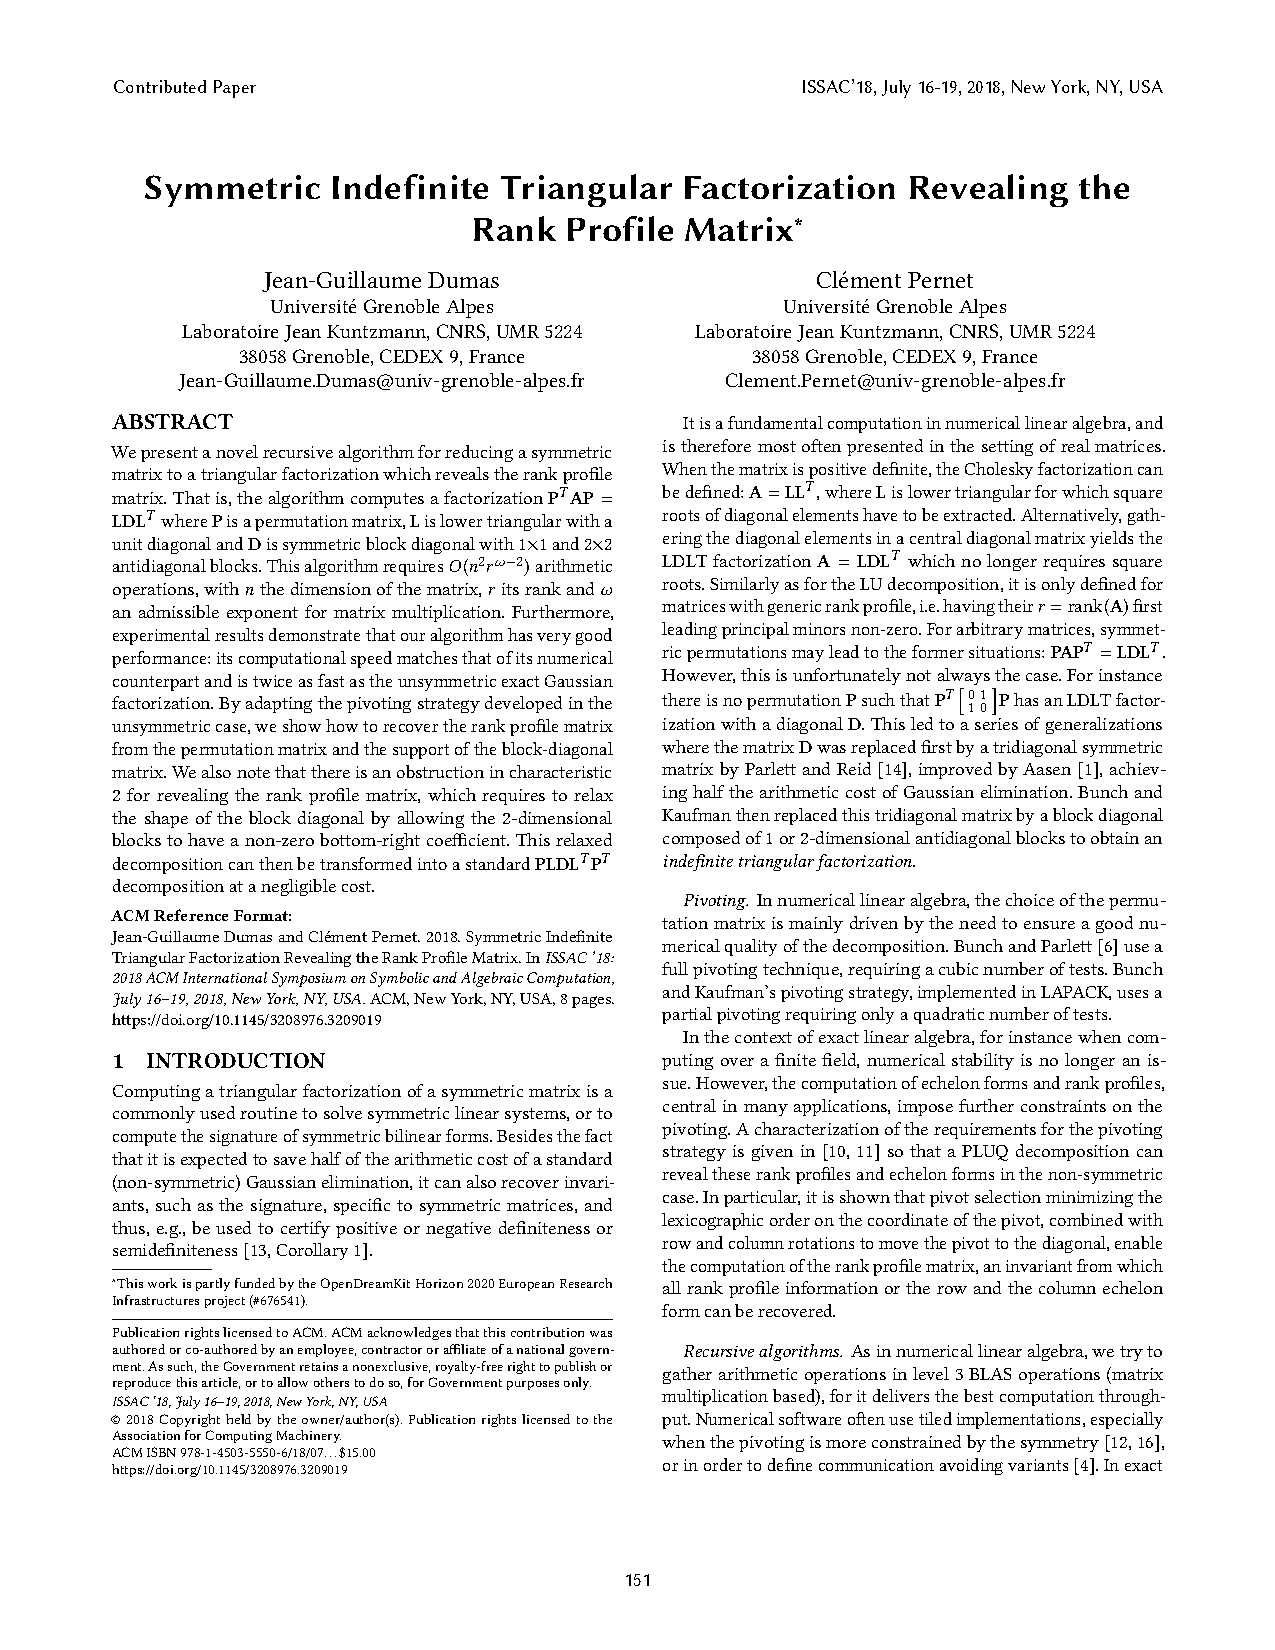
\includepdf[pages={1-8}]{DumasPernet18.pdf}

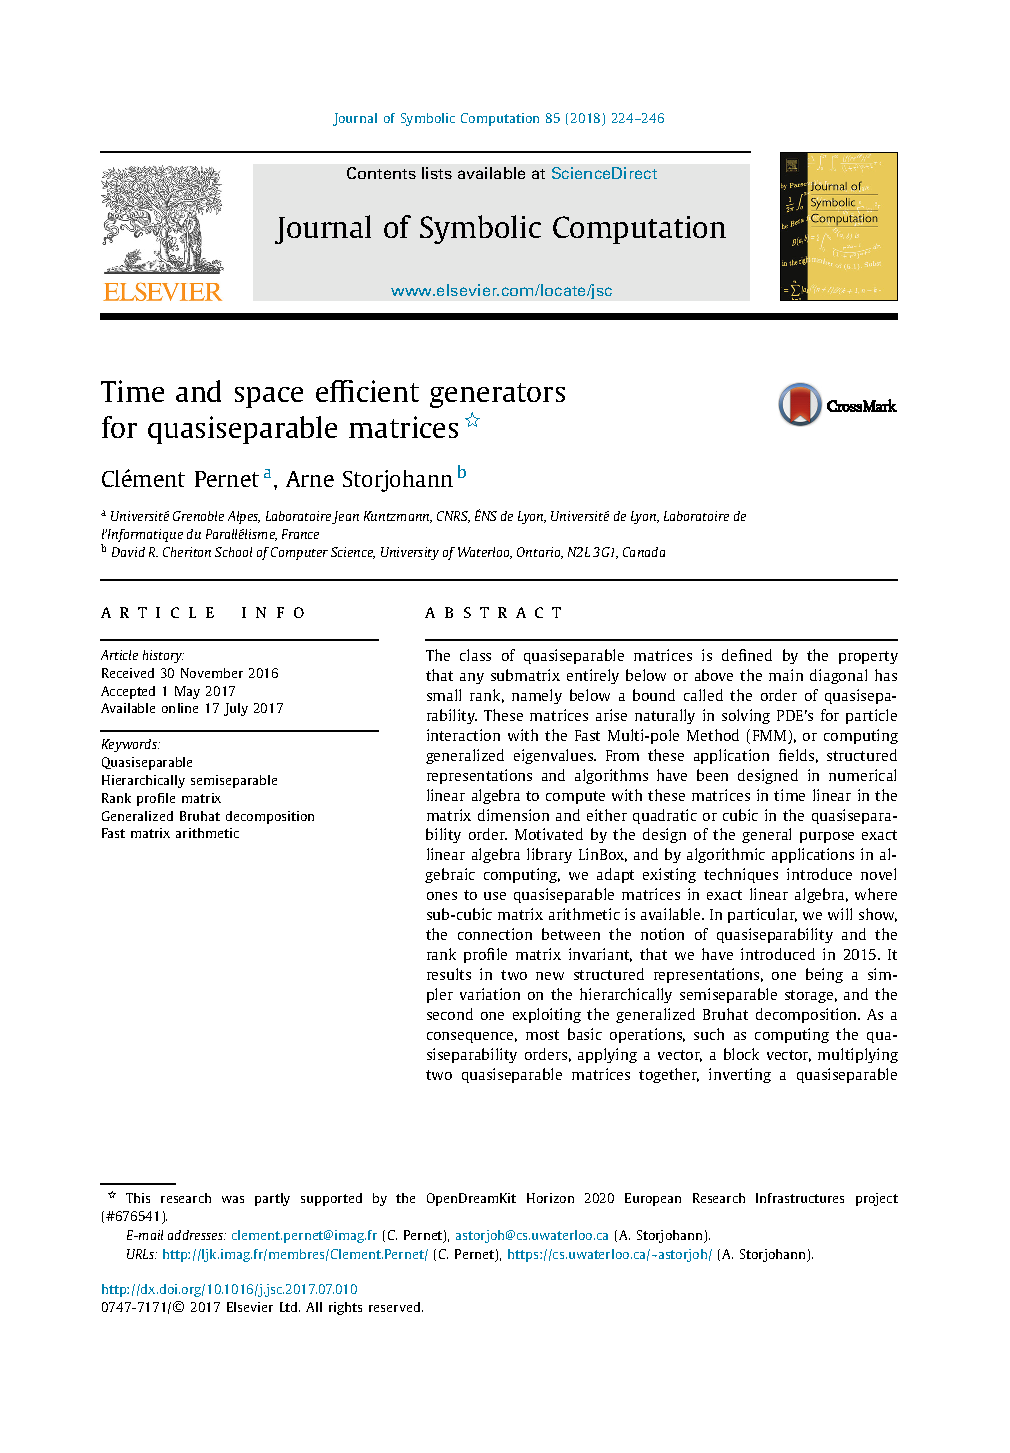
\includepdf[pages={1-23}]{PernetStorjohann18.pdf}

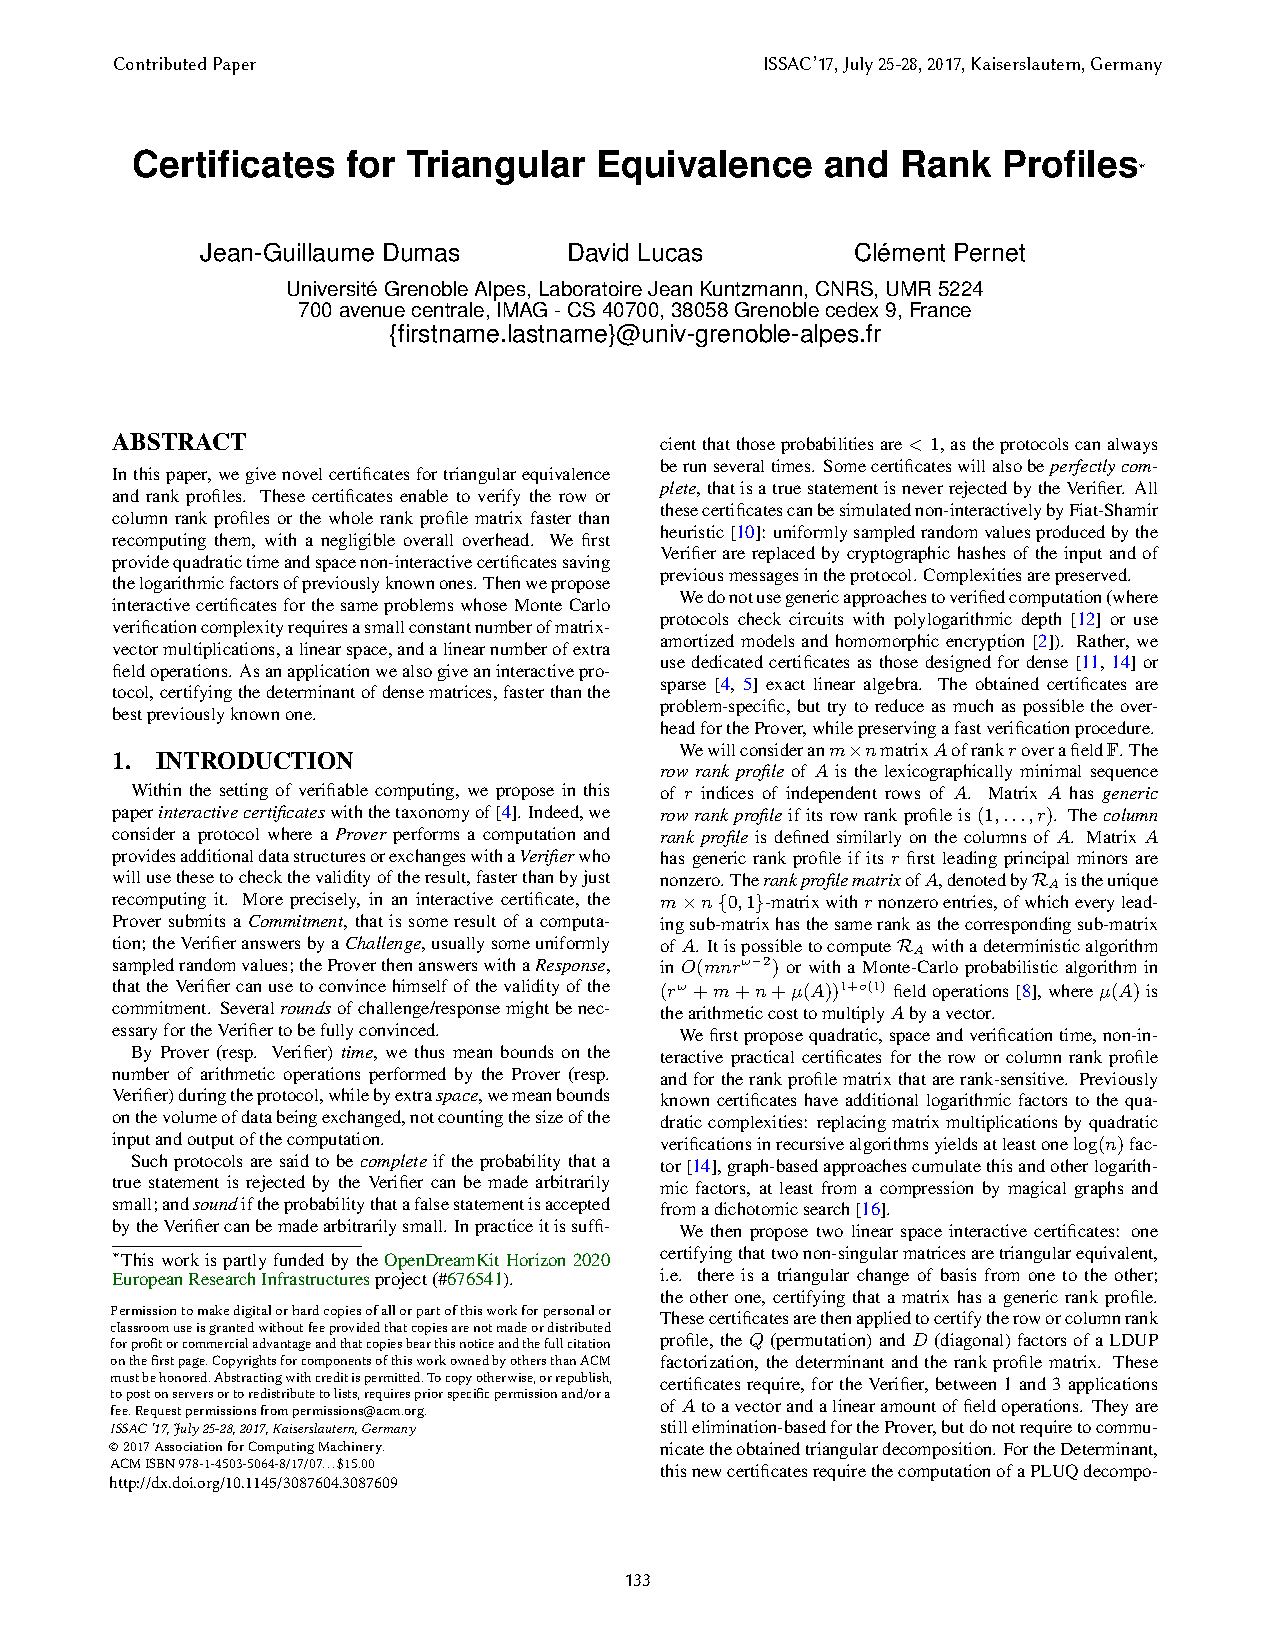
\includepdf[pages={1-8}]{DLP18.pdf}

\end{document}

%%% Local Variables:
%%% mode: latex
%%% mode: flyspell
%%% ispell-local-dictionary: "american"
%%% TeX-master: t
%%% End:

